\section{ Introduction et objectifs}
\subsection{Objectifs}
Nous repartons du projet où nous l'avons laissé. Nous allons ajouter des filtres pour notre boutique : une barre de recherche, un filtre par prix et un filtre par catégorie.

\subsection{Création de l'interface pour nos filtres}
Dans le dossier {\tt interfaces}, créez le fichier {\tt Filters.interface.ts} :
\begin{minted}[
mathescape,
framesep=2mm,
baselinestretch=1.2,
fontsize=\footnotesize,
bgcolor=LightGray,
%linenos
]{javascript}
export type Category = 'gamer' | 'desktop' | 'streaming' | 'all';

export interface FiltersInterface {
  search: string;
  priceRange: [number, number];
  category: Category;
}
\end{minted}
Modifiez ensuite les {\color{monOrange}exports} de l'{\tt index} :
\begin{minted}[
mathescape,
framesep=2mm,
baselinestretch=1.2,
fontsize=\footnotesize,
bgcolor=LightGray,
%linenos
]{javascript}
export * from './Product.interface';
export * from './ProductCart.interface';
export * from './Filters.interface';
\end{minted}
\subsection{Modification de {\color{monOrange}App.vue}}
Nous modifions le {\color{monOrange}state} réactif de notre composant racine, en ajoutant une propriété qui contient les filtres en cours. Nous avons des filtres sélectionnés par défaut contenus dans {\tt DEFAULT\_FILTERS}.
\begin{minted}[
mathescape,
framesep=2mm,
baselinestretch=1.2,
fontsize=\footnotesize,
bgcolor=LightGray,
%linenos
]{javascript}
<script setup lang="ts">
import TheHeader from './components/Header.vue';
import TheFooter from './components/Footer.vue';
import Shop from './components/Shop/Shop.vue';
import Cart from './components/Cart/Cart.vue';
import data from './data/product';
import { DEFAULT_FILTERS } from './data/filters';
import { computed, reactive } from 'vue';
import type {
  FiltersInterface,
  ProductCartInterface,
  ProductInterface,
} from './interfaces';

const state = reactive<{
  products: ProductInterface[];
  cart: ProductCartInterface[];
  filters: FiltersInterface;
}>({
  products: data,
  cart: [],
  filters: DEFAULT_FILTERS,
});
// …
\end{minted}
\subsection{Création du fichier {\tt data/filters.ts}}
Nous exportons nos filtres par défaut dans une constante :
\begin{minted}[
mathescape,
framesep=2mm,
baselinestretch=1.2,
fontsize=\footnotesize,
bgcolor=LightGray,
%linenos
]{javascript}
import type { FiltersInterface } from '../interfaces';

export const DEFAULT_FILTERS: FiltersInterface = {
  search: '',
  priceRange: [0, 10000],
  category: 'all',
};
\end{minted}
\subsection{Modification de l'interface Product}
Modifiez le fichier {\tt interfaces/ProductInterface.ts} pour ajouter une propriété {\color{monOrange}category} :
\begin{minted}[
mathescape,
framesep=2mm,
baselinestretch=1.2,
fontsize=\footnotesize,
bgcolor=LightGray,
%linenos
]{javascript}
import type { Category } from './Filters.interface';

export interface ProductInterface {
  id: number;
  title: string;
  image: string;
  price: number;
  description: string;
  category: Category;
}
\end{minted}
\subsection{Modification de data/products}
Il faut ajouter ensuite une catégorie à nos produits en dur :
\begin{minted}[
mathescape,
framesep=2mm,
baselinestretch=1.2,
fontsize=\footnotesize,
bgcolor=LightGray,
%linenos
]{javascript}
import type { ProductInterface } from "@/interfaces";

export default [
    {
        id: 1,
        image: 'src/assets/images/macbookpro.PNG',
        title: 'Macbook Pro',
        description: 'Lorem ipsum dolor sit amet consectetur adipisicing edolor tempore ipsam cum ipsum reiciendis',
        price: 1500,
        category: 'desktop'
    },
    {
        id: 2,
        image: 'src/assets/images/levono.PNG',
        title: 'Levono Pro',
        description: 'Lorem ipsum dolor sit amet consectetur adipisicing edolor tempore ipsam cum ipsum reiciendis',
        price: 2300,
        category: 'desktop'
    },
    {
        id: 3,
        image: 'src/assets/images/rider.PNG',
        title: 'Rider',
        description: 'Lorem ipsum dolor sit amet consectetur adipisicing edolor tempore ipsam cum ipsum reiciendis',
        price: 1200,
        category: 'gamer'
    },
    {
        id: 4,
        image: 'src/assets/images/ldlc.PNG',
        title: 'LDLC benolo',
        description: 'Lorem ipsum dolor sit amet consectetur adipisicing edolor tempore ipsam cum ipsum reiciendis',
        price: 4500,
        category: 'streaming'
    },
    {
        id: 5,
        image: 'src/assets/images/asus.PNG',
        title: 'Asus gamer',
        description: 'Lorem ipsum dolor sit amet consectetur adipisicing edolor tempore ipsam cum ipsum reiciendis',
        price: 3755,
        category: 'gamer'
    },
    {
        id: 6,
        image: 'src/assets/images/rog.PNG',
        title: 'Rog desktop',
        description: 'Lorem ipsum dolor sit amet consectetur adipisicing edolor tempore ipsam cum ipsum reiciendis',
        price: 2452,
        category: 'streaming'
    },
    {
        id: 7,
        image: 'src/assets/images/msi.PNG',
        title: 'MSI play',
        description: 'Lorem ipsum dolor sit amet consectetur adipisicing edolor tempore ipsam cum ipsum reiciendis',
        price: 1478,
        category: 'gamer'
    },
    {
        id: 8,
        image: 'src/assets/images/pad.PNG',
        title: 'Think pad',
        description: 'Lorem ipsum dolor sit amet consectetur adipisicing edolor tempore ipsam cum ipsum reiciendis',
        price: 899,
        category: 'desktop'
    },
] as ProductInterface[]
\end{minted}
Code de la vidéo
Voici le code de la vidéo :

%%%%%%%%%%%%%%%%%%%%%%%%%%%%%%%%%%%%%%%%%%%%%%%%%%%%%%%%%%%%%%%%%%%%%

\section{Préparation pour le filtrage des produits}
\subsection{Modification de ShopProductList.vue}
Nous ajoutons une {\color{monOrange}key} pour la directive {\color{monOrange}v-for} afin d'optimiser les performances de mise à jour des produits :
\begin{minted}[
mathescape,
framesep=2mm,
baselinestretch=1.2,
fontsize=\footnotesize,
bgcolor=LightGray,
%linenos
]{html}
<script setup lang="ts">
import type { ProductInterface } from '@/interfaces';
import ShopProduct from './ShopProduct.vue';

defineProps<{
  products: ProductInterface[];
}>();

const emit = defineEmits<{
  (e: 'addProductToCart', productId: number): void;
}>();
</script>

<template>
  <div class="grid p-20">
    <ShopProduct
      @add-product-to-cart="emit('addProductToCart', $event)"
      v-for="product of products"
      :product="product"
      :key="product.id"
    />
  </div>
</template>

<style lang="scss" scoped>
.grid {
  display: grid;
  grid-template-columns: 1fr 1fr 1fr 1fr;
  grid-auto-rows: 400px;
  gap: 20px;
}
</style>
\end{minted}
%$
\subsection{Modification de Filters.interface.ts}
Nous allons ajouter une interface {\tt FilterUpdate} :
\begin{minted}[
mathescape,
framesep=2mm,
baselinestretch=1.2,
fontsize=\footnotesize,
bgcolor=LightGray,
%linenos
]{javascript}
export type Category = 'gamer' | 'desktop' | 'streaming' | 'all';

export interface FiltersInterface {
  search: string;
  priceRange: [number, number];
  category: Category;
}

export interface FilterUpdate {
  search?: string;
  priceRange?: [number, number];
  category?: Category;
}
\end{minted}
{\tt FilterUpdate} contiendra le filtre appliqués par l'utilisateur à chaque fois qu'il modifie un filtre. Ainsi par exemple, s'il modifie l'intervalle de prix, l'objet contiendra {\tt priceRange} uniquement. Même chose s'il effectue une recherche, nous aurons la propriété {\color{monOrange}search} uniquement. C'est pour cette raison que toutes les propriétés sont optionnelles avec {\color{monOrange}?}.

\subsection{Modification de {\tt App.vue}}
Nous filtrons les produits à afficher en fonction de toutes les options des filtres que nous allons mettre en place en utilisant une propriété calculée. Nous écoutons l'événement que nous allons émettre lorsque l'utilisateur modifiera un filtre et nous modifions l'état des filtres en fonction de l'événement reçu.
\begin{minted}[
mathescape,
framesep=2mm,
baselinestretch=1.2,
fontsize=\footnotesize,
bgcolor=LightGray,
%linenos
]{html}
<script setup lang="ts">
import TheHeader from './components/Header.vue';
import TheFooter from './components/Footer.vue';
import Shop from './components/Shop/Shop.vue';
import Cart from './components/Cart/Cart.vue';
import data from './data/product';
import { computed, reactive } from 'vue';
import type {
  FiltersInterface,
  ProductCartInterface,
  ProductInterface,
  FilterUpdate,
} from './interfaces';
import { DEFAULT_FILTERS } from './data/filters';

const state = reactive<{
  products: ProductInterface[];
  cart: ProductCartInterface[];
  filters: FiltersInterface;
}>({
  products: data,
  cart: [],
  filters: { ...DEFAULT_FILTERS },
});

function addProductToCart(productId: number): void {
  const product = state.products.find((product) => product.id === productId);
  if (product) {
    const productInCart = state.cart.find(
      (product) => product.id === productId
    );
    if (productInCart) {
      productInCart.quantity++;
    } else {
      state.cart.push({ ...product, quantity: 1 });
    }
  }
}

function removeProductFromCart(productId: number): void {
  const productFromCart = state.cart.find(
    (product) => product.id === productId
  );
  if (productFromCart?.quantity === 1) {
    state.cart = state.cart.filter((product) => product.id !== productId);
  } else {
    productFromCart.quantity--;
  }
}

function updateFilter(filterUpdate: FilterUpdate) {
  if (filterUpdate.search !== undefined) {
    state.filters.search = filterUpdate.search;
  } else if (filterUpdate.priceRange) {
    state.filters.priceRange = filterUpdate.priceRange;
  } else if (filterUpdate.category) {
    state.filters.category = filterUpdate.category;
  } else {
    state.filters = { ...DEFAULT_FILTERS };
  }
}

const cartEmpty = computed(() => state.cart.length === 0);

const filteredProducts = computed(() => {
  return state.products.filter((product) => {
    if (
      product.title
        .toLocaleLowerCase()
        .startsWith(state.filters.search.toLocaleLowerCase()) &&
      product.price >= state.filters.priceRange[0] &&
      product.price <= state.filters.priceRange[1] &&
      (product.category === state.filters.category ||
        state.filters.category === 'all')
    ) {
      return true;
    } else {
      return false;
    }
  });
});
</script>

<template>
  <div
    class="app-container"
    :class="{
      gridEmpty: cartEmpty,
    }"
  >
    <TheHeader class="header" />
    <Shop
      @update-filter="updateFilter"
      :products="filteredProducts"
      @add-product-to-cart="addProductToCart"
      class="shop"
    />
    <Cart
      v-if="!cartEmpty"
      :cart="state.cart"
      class="cart"
      @remove-product-from-cart="removeProductFromCart"
    />
    <TheFooter class="footer" />
  </div>
</template>
\end{minted}
Notez bien que nous passons maintenant la propriété calculée {\tt filteredProducts} à notre composant Shop et non plus les produits du {\color{monOrange}state}.

Notez également que {\tt \{ ...DEFAULT\_FILTERS \} } permet de créer un nouvel objet différent lors de la réinitialisation des filtres pour ne pas avoir le même objet que dans le {\color{monOrange}state}.

\subsection{Code de la vidéo}
Voici le code de la vidéo :

%%%%%%%%%%%%%%%%%%%%%%%%%%%%%%%%%%%%%%%%%%%%%%%%%%%%%%%%%%%%%%%%%%%%%
\section{Création du composant ShopFilters}
\subsection{Création du composantShopFilters}
Dans le dossier {\tt src/shop} créez le fichier {\tt ShopFilters.vue}. Ce sera le composant responsable des filtres de l’application.

\subsection{Modification deApp.vue}
Nous passons en {\color{monOrange}prop} les filtres à notre composant {\color{monOrange}Shop} pour que celui-ci puisse les passer ensuite au composant responsable des filtres.
\begin{minted}[
mathescape,
framesep=2mm,
baselinestretch=1.2,
fontsize=\footnotesize,
bgcolor=LightGray,
%linenos
]{html}
<template>
  <div
    class="app-container"
    :class="{
      gridEmpty: cartEmpty,
    }"
  >
    <TheHeader class="header" />
    <Shop
      @update-filter="updateFilter"
      :products="filteredProducts"
      :filters="state.filters"
      @add-product-to-cart="addProductToCart"
      class="shop"
    />
    <!-- ..... -->
\end{minted}
\subsection{Modification de Shop.vue}
Nous modifions le composant {\tt Shop.vue} qui va recevoir en {\color{monOrange}prop} les filtres depuis le composant {\tt App.vue}. Il les repasse ensuite au composant {\tt ShopFilters}. Il va également ré-émettre l'événement {\tt updateFilter} qu'il va recevoir du composant {\tt ShopFilters} pour mettre à jour le filtre modifié par l'utilisateur. Ici il ne fait donc que transmettre l'événement et les {\color{monOrange}props} dans les deux sens entre {\tt App.vue} et {\tt ShopFilters}.
\begin{minted}[
mathescape,
framesep=2mm,
baselinestretch=1.2,
fontsize=\footnotesize,
bgcolor=LightGray,
%linenos
]{html}
<script setup lang="ts">
import type {
  FiltersInterface,
  ProductInterface,
  FilterUpdate,
} from '../../interfaces';
import ShopProductList from './ShopProductList.vue';
import ShopFilters from './ShopFilters.vue';

defineProps<{
  products: ProductInterface[];
  filters: FiltersInterface;
}>();

const emit = defineEmits<{
  (e: 'addProductToCart', productId: number): void;
  (e: 'updateFilter', updateFilter: FilterUpdate): void;
}>();
</script>

<template>
  <div class="d-flex flex-row">
    <ShopFilters
      :filters="filters"
      @update-filter="emit('updateFilter', $event)"
      class="shop-filter"
    />
    <ShopProductList
      class="flex-fill"
      @add-product-to-cart="emit('addProductToCart', $event)"
      :products="products"
    />
  </div>
</template>

<style lang="scss" scoped>
.shop-filter {
  flex: 0 0 200px;
}
</style>
\end{minted}
\subsection{Modification de {\tt ShopFilters.vue}}
Nous mettons en place le composant en créant le premier filtre pour la recherche par nom de produit. Lorsque l'utilisateur tape dans le champ de la recherche, il va émettre un événement {\tt updateFilter} avec la valeur du champ.
\begin{minted}[
mathescape,
framesep=2mm,
baselinestretch=1.2,
fontsize=\footnotesize,
bgcolor=LightGray,
%linenos
]{html}
<script setup lang="ts">
import type { FiltersInterface, FilterUpdate } from '../../interfaces';
defineProps<{
  filters: FiltersInterface;
}>();
const emit = defineEmits<{
  (e: 'updateFilter', filterUpdate: FilterUpdate): void;
}>();
</script>

<template>
  <div class="p-20 d-flex flex-column">
    <section class="mb-20">
      <h3 class="mb-10">Rechercher</h3>
      <input
        :value="filters.search"
        @input="emit('updateFilter', { search: ($event.target as HTMLInputElement).value })"
        type="text"
        placeholder="Rechercher"
      />
    </section>
  </div>
</template>

<style lang="scss" scoped></style>
\end{minted}

% $%Code de la vidéo 
%Voici le code de la vidéo :

\begin{center}
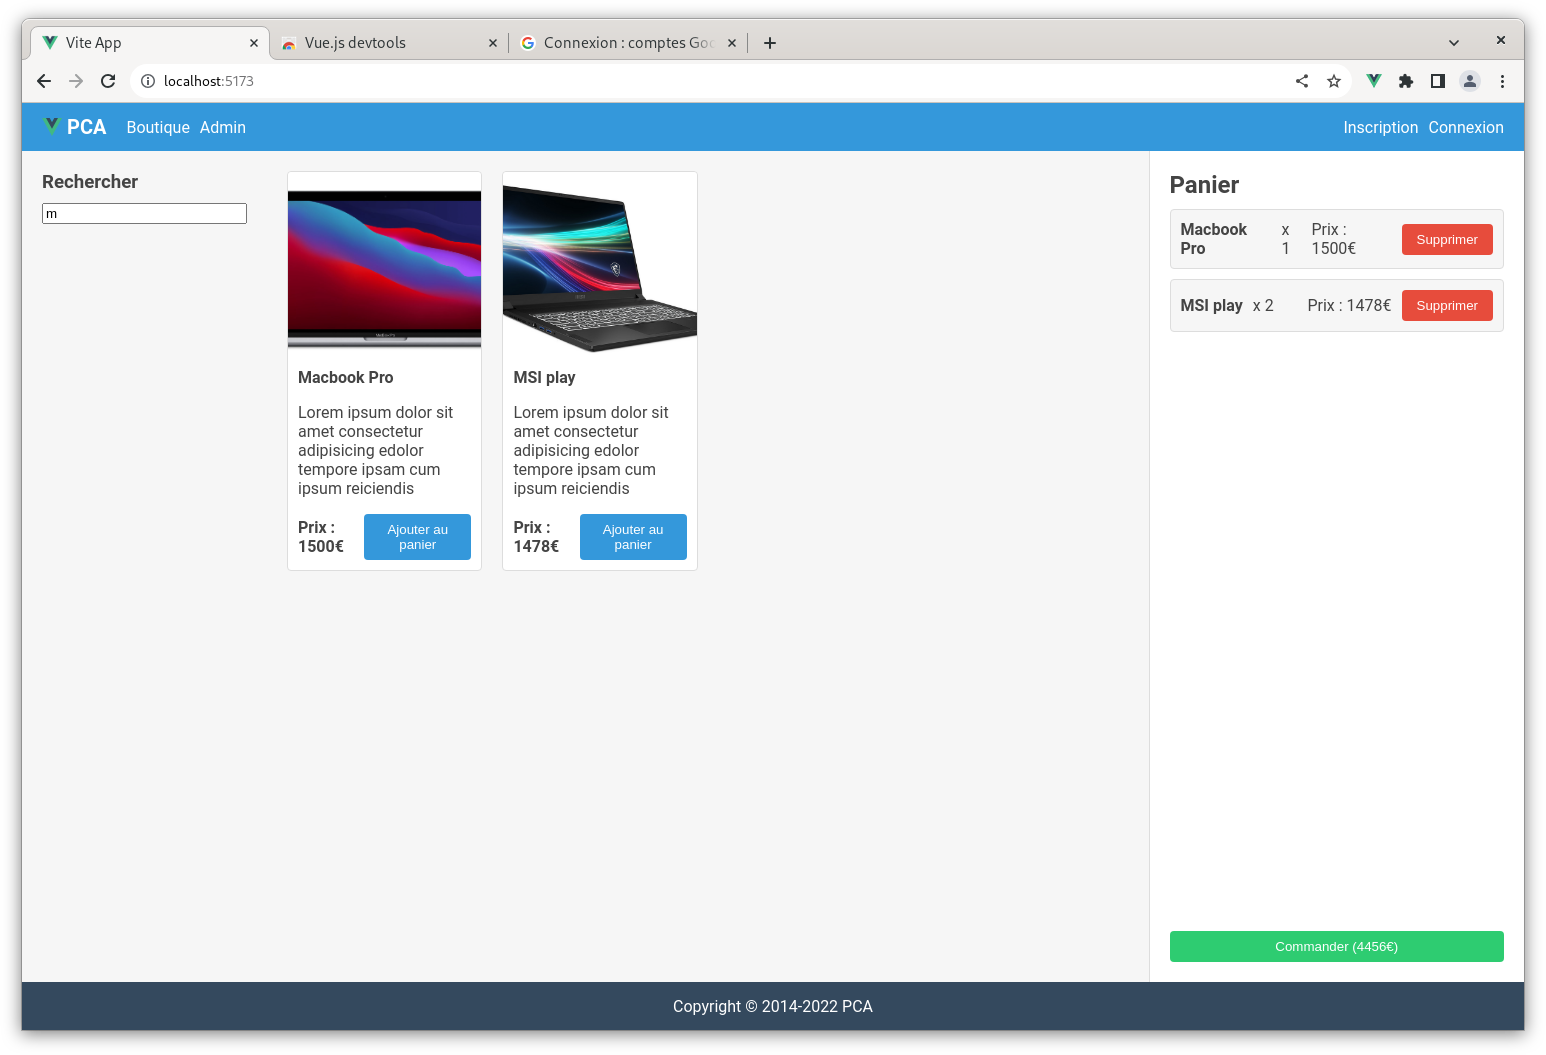
\includegraphics[width=15cm]{images/image25.png}
\end{center}
%%%%%%%%%%%%%%%%%%%%%%%%%%%%%%%%%%%%%%%%%%%%%%%%%%%%%%%%%%%%%%%%%%%%%

\section{Filtrer les produits par prix}
\subsection{Modification de {\tt ShopFilters.vue}}
Nous ajoutons le filtre par intervalles de prix :
\begin{minted}[
mathescape,
framesep=2mm,
baselinestretch=1.2,
fontsize=\footnotesize,
bgcolor=LightGray,
%linenos
]{html}
<script setup lang="ts">
import type { FiltersInterface, FilterUpdate } from '../../interfaces';
defineProps<{
  filters: FiltersInterface;
}>();
const emit = defineEmits<{
  (e: 'updateFilter', filterUpdate: FilterUpdate): void;
}>();
</script>

<template>
  <div class="p-20 d-flex flex-column">
    <section class="mb-20">
      <h3 class="mb-10">Rechercher</h3>
      <input
        :value="filters.search"
        @input="emit('updateFilter', { search: ($event.target as HTMLInputElement).value })"
        type="text"
        placeholder="Rechercher"
      />
    </section>
    <section class="mb-20">
      <h3 class="mb-10">Trier par prix</h3>
      <div
        class="mb-5"
        v-for="priceRange of ([[0, 10000], [800, 1000], [1000, 1500], [1500, 2000], [2000, 10000]] as [number, number][])"
      >
        <input
          :checked="filters.priceRange[0] === priceRange[0]"
          type="radio"
          @input="emit('updateFilter', { priceRange })"
          name="priceRange"
          :id="priceRange[0].toString()"
        />
        <label :for="priceRange[0].toString()">
          {{
            priceRange[0] === 0
              ? 'Tous les prix'
              : priceRange[0] === 2000
              ? 'Plus de 2000€'
              : `Entre ${priceRange[0]}€ et ${priceRange[1]}€`
          }}
        </label>
      </div>
    </section>
  </div>
</template>

<style lang="scss" scoped></style>
\end{minted}

%$
\begin{itemize}
\item {\color{monOrange} as [number, number][]:} permet de préciser à TypeScriptque nous avons bien un tableau contenant des tableaux avec exactement deux éléments de type nombre.

\item {\color{monOrange} v-for="priceRange of:} permet d'itérer sur l'ensemble des intervalles de prix.

\item {\color{monOrange} :checked="filters.priceRange[0] === priceRange[0]":} nous cochons l'élément uniquement si la valeur minimale de l'intervalle contenue dans les filtres passés est la même que la valeur minimale de l'intervalle de l'itération en cours.

\item {\color{monOrange} @input="emit('updateFilter', { priceRange })": } permet d'émettre l'événement de mise à jour des filtres avec en valeur un objet contenant une propriété qui a en clé le filtre à modifier et en valeur l'intervalle sélectionné.

\item {\color{monOrange} :id="priceRange[0].toString()":} nous nous servions de la valeur Inférieure de l'intervalle comme identifiant HTMLunique.

\end{itemize}
\subsection{Code de la vidéo}
Voici le code de la vidéo :

\begin{center}
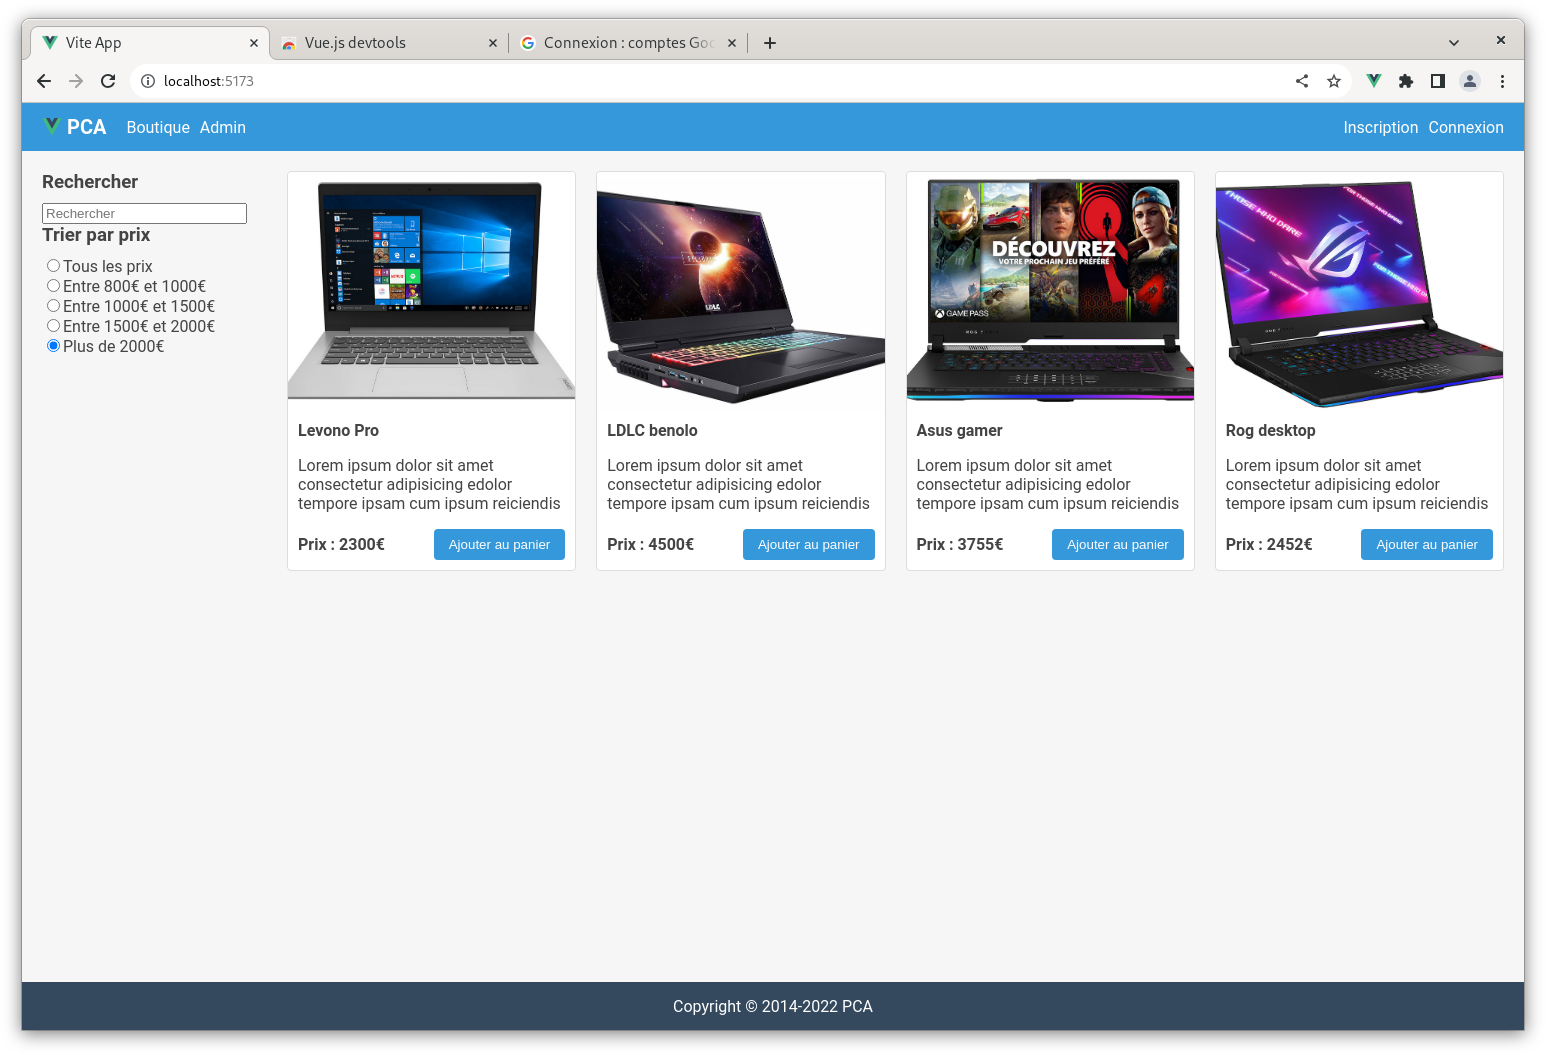
\includegraphics[width=15cm]{images/image26.png}
\end{center}

%%%%%%%%%%%%%%%%%%%%%%%%%%%%%%%%%%%%%%%%%%%%%%%%%%%%%%%%%%%%%%%%%%%%%%%
\section{Filtrer les produits par catégorie}
\subsection{Modification de {\tt ShopFilters.vue}}
Nous ajoutons le filtre par catégorie :
\begin{minted}[
mathescape,
framesep=2mm,
baselinestretch=1.2,
fontsize=\footnotesize,
bgcolor=LightGray,
%linenos
]{html}
<script setup lang="ts">
import type {
  FiltersInterface,
  FilterUpdate,
  Category,
} from '../../interfaces';
defineProps<{
  filters: FiltersInterface;
}>();
const emit = defineEmits<{
  (e: 'updateFilter', filterUpdate: FilterUpdate): void;
}>();
</script>

<template>
  <div class="p-20 d-flex flex-column">
    <section class="mb-20">
      <h3 class="mb-10">Rechercher</h3>
      <input
        :value="filters.search"
        @input="emit('updateFilter', { search: ($event.target as HTMLInputElement).value })"
        type="text"
        placeholder="Rechercher"
      />
    </section>
    <section class="mb-20">
      <h3 class="mb-10">Trier par prix</h3>
      <div
        class="mb-5"
        v-for="priceRange of ([[0, 10000], [800, 1000], [1000, 1500], [1500, 2000], [2000, 10000]] as [number, number][])"
      >
        <input
          :checked="filters.priceRange[0] === priceRange[0]"
          type="radio"
          @input="emit('updateFilter', { priceRange })"
          name="priceRange"
          :id="priceRange[0].toString()"
        />
        <label :for="priceRange[0].toString()">
          {{
            priceRange[0] === 0
              ? 'Tous les prix'
              : priceRange[0] === 2000
              ? 'Plus de 2000€'
              : `Entre ${priceRange[0]}€ et ${priceRange[1]}€`
          }}
        </label>
      </div>
    </section>
    <section class="mb-20 flex-fill">
      <h3 class="mb-10">Trier par categories</h3>
      <p
        class="category"
        :class="{ selected: filters.category === category }"
        v-for="category in (['all', 'desktop', 'gamer', 'streaming'] as Category[])"
        @click="emit('updateFilter', { category })"
      >
        {{ category }}
      </p>
    </section>
  </div>
</template>

<style lang="scss" scoped>
.category {
  font-size: 14px;
  line-height: 18px;
  cursor: pointer;
  &:hover {
    text-decoration: underline;
  }
}
.selected {
  font-weight: bold;
  text-decoration: underline;
}
</style>
\end{minted}

%$
{\color{monOrange} :class="{ selected: filters.category === category }":} permet d'ajouter la classe {\tt selected} si la catégorie sélectionnée dans la {\color{monOrange} props} {\tt filters} est celle de l'itération en cours.

\subsection{Code de la vidéo}
Voici le code de la vidéo :
\begin{center}
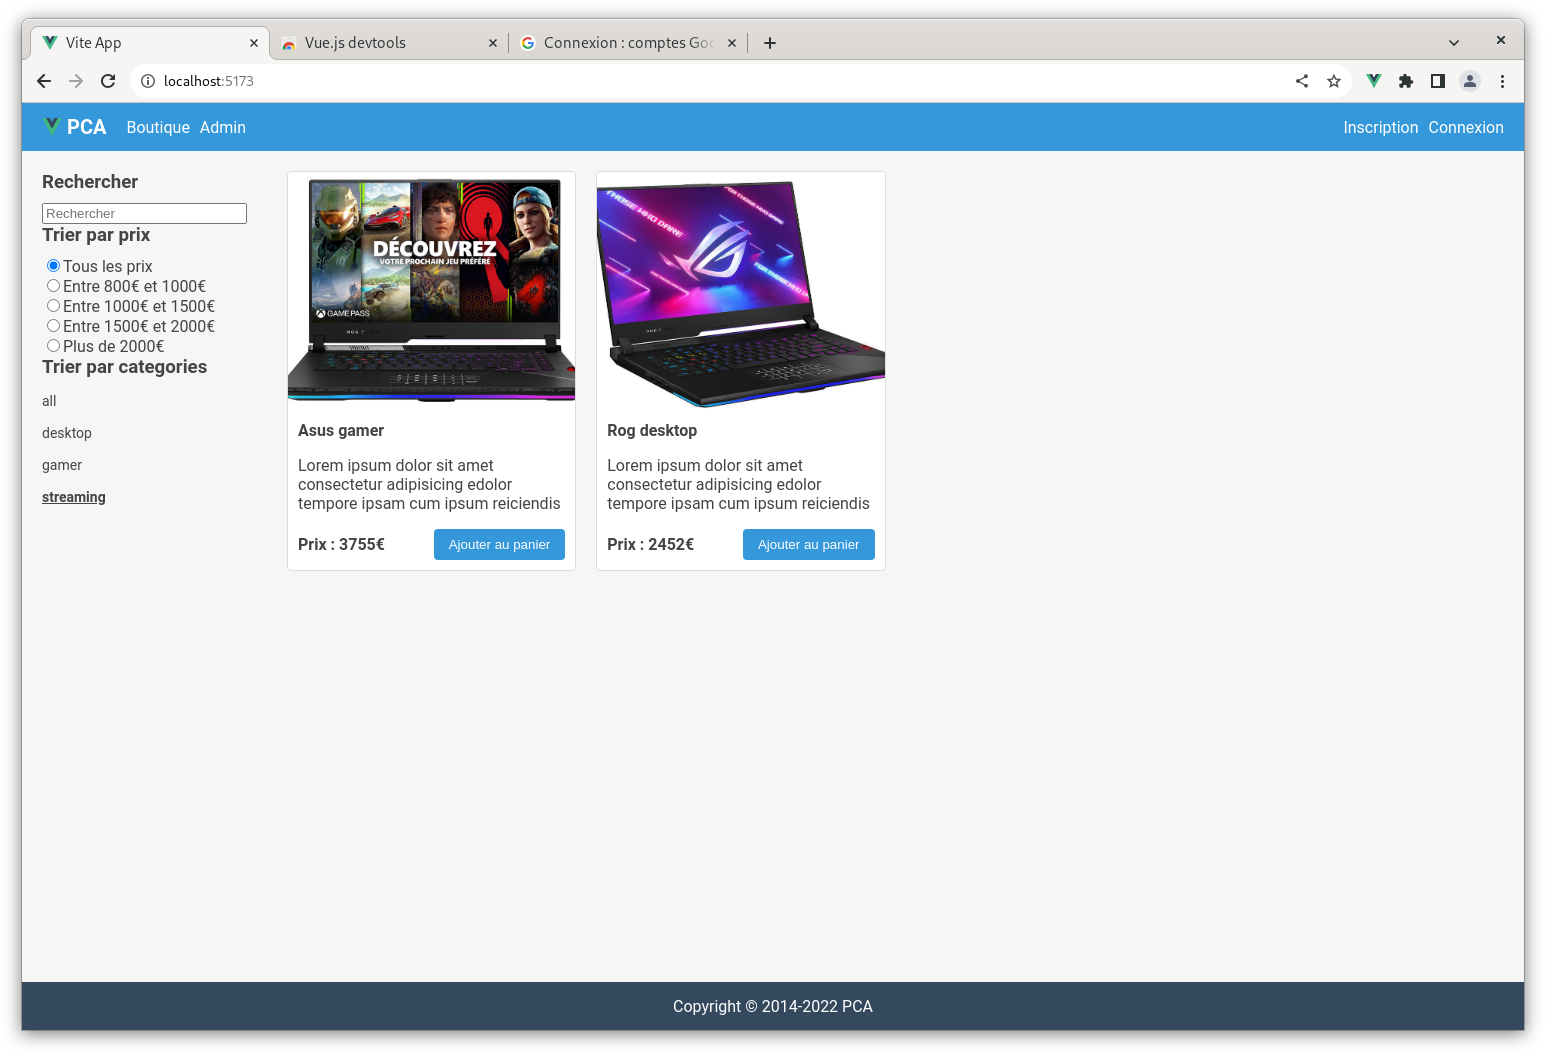
\includegraphics[width=15cm]{images/image27.png}
\end{center}
%%%%%%%%%%%%%%%%%%%%%%%%%%%%%%%%%%%%%%%%%%%%%%%%%%%%%%%%%%%%%%%%%%%%%%%

\section{Reset des filtres}
\subsection{Modification de {\tt ShopFilters.vue}}
Nous ajoutons la reset des filtres et l'affichage du nombre de résultat :
\begin{minted}[
mathescape,
framesep=2mm,
baselinestretch=1.2,
fontsize=\footnotesize,
bgcolor=LightGray,
%linenos
]{html}
<script setup lang="ts">
import type {
  FiltersInterface,
  FilterUpdate,
  Category,
} from '../../interfaces';
defineProps<{
  filters: FiltersInterface;
  nbrOfProducts: number;
}>();
const emit = defineEmits<{
  (e: 'updateFilter', filterUpdate: FilterUpdate): void;
}>();
</script>

<template>
  <div class="p-20 d-flex flex-column">
    <section class="mb-20">
      <h3 class="mb-10">Rechercher</h3>
      <input
        :value="filters.search"
        @input="emit('updateFilter', { search: ($event.target as HTMLInputElement).value })"
        type="text"
        placeholder="Rechercher"
      />
    </section>
    <section class="mb-20">
      <h3 class="mb-10">Trier par prix</h3>
      <div
        class="mb-5"
        v-for="priceRange of ([[0, 10000], [800, 1000], [1000, 1500], [1500, 2000], [2000, 10000]] as [number, number][])"
      >
        <input
          :checked="filters.priceRange[0] === priceRange[0]"
          type="radio"
          @input="emit('updateFilter', { priceRange })"
          name="priceRange"
          :id="priceRange[0] + ''"
        />
        <label :for="priceRange[0] + ''">
          {{
            priceRange[0] === 0
              ? 'Tous les prix'
              : priceRange[0] === 2000
              ? 'Plus de 2000€'
              : `Entre ${priceRange[0]}€ et ${priceRange[1]}€`
          }}
        </label>
      </div>
    </section>
    <section class="mb-20 flex-fill">
      <h3 class="mb-10">Trier par categories</h3>
      <p
        class="category"
        :class="{ selected: filters.category === category }"
        v-for="category in (['all', 'desktop', 'gamer', 'streaming'] as Category[])"
        @click="emit('updateFilter', { category })"
      >
        {{ category }}
      </p>
    </section>
    <small class="mb-5">
      Nombre de résultats:
      <strong>{{ nbrOfProducts }}</strong>
    </small>
    <button class="btn btn-danger" @click="emit('updateFilter', {})">
      Supprimer les filtres
    </button>
  </div>
</template>

<style lang="scss" scoped>
.category {
  font-size: 14px;
  line-height: 18px;
  cursor: pointer;
  &:hover {
    text-decoration: underline;
  }
}
.selected {
  font-weight: bold;
  text-decoration: underline;
}
</style>

\end{minted}

% $
\subsection{Modification de {\tt Shop.vue}}
Il ne faut pas oublier de modifier le composant {\color{monOrange} Shop} pour passer en {\color{monOrange} prop} le nombre de résultats :
\begin{minted}[
mathescape,
framesep=2mm,
baselinestretch=1.2,
fontsize=\footnotesize,
bgcolor=LightGray,
%linenos
]{html}
<script setup lang="ts">
import type {
  FiltersInterface,
  ProductInterface,
  FilterUpdate,
} from '../../interfaces';
import ShopProductList from './ShopProductList.vue';
import ShopFilters from './ShopFilters.vue';

defineProps<{
  products: ProductInterface[];
  filters: FiltersInterface;
}>();

const emit = defineEmits<{
  (e: 'addProductToCart', productId: number): void;
  (e: 'updateFilter', updateFilter: FilterUpdate): void;
}>();
</script>

<template>
  <div class="d-flex flex-row">
    <ShopFilters
      :filters="filters"
      :nbr-of-products="products.length"
      @update-filter="emit('updateFilter', $event)"
      class="shop-filter"
    />
    <ShopProductList
      class="flex-fill"
      @add-product-to-cart="emit('addProductToCart', $event)"
      :products="products"
    />
  </div>
</template>

<style lang="scss" scoped>
.shop-filter {
  flex: 0 0 200px;
}
</style>
\end{minted}
Code de la vidéo
Voici le code de la vidéo :
\begin{center}
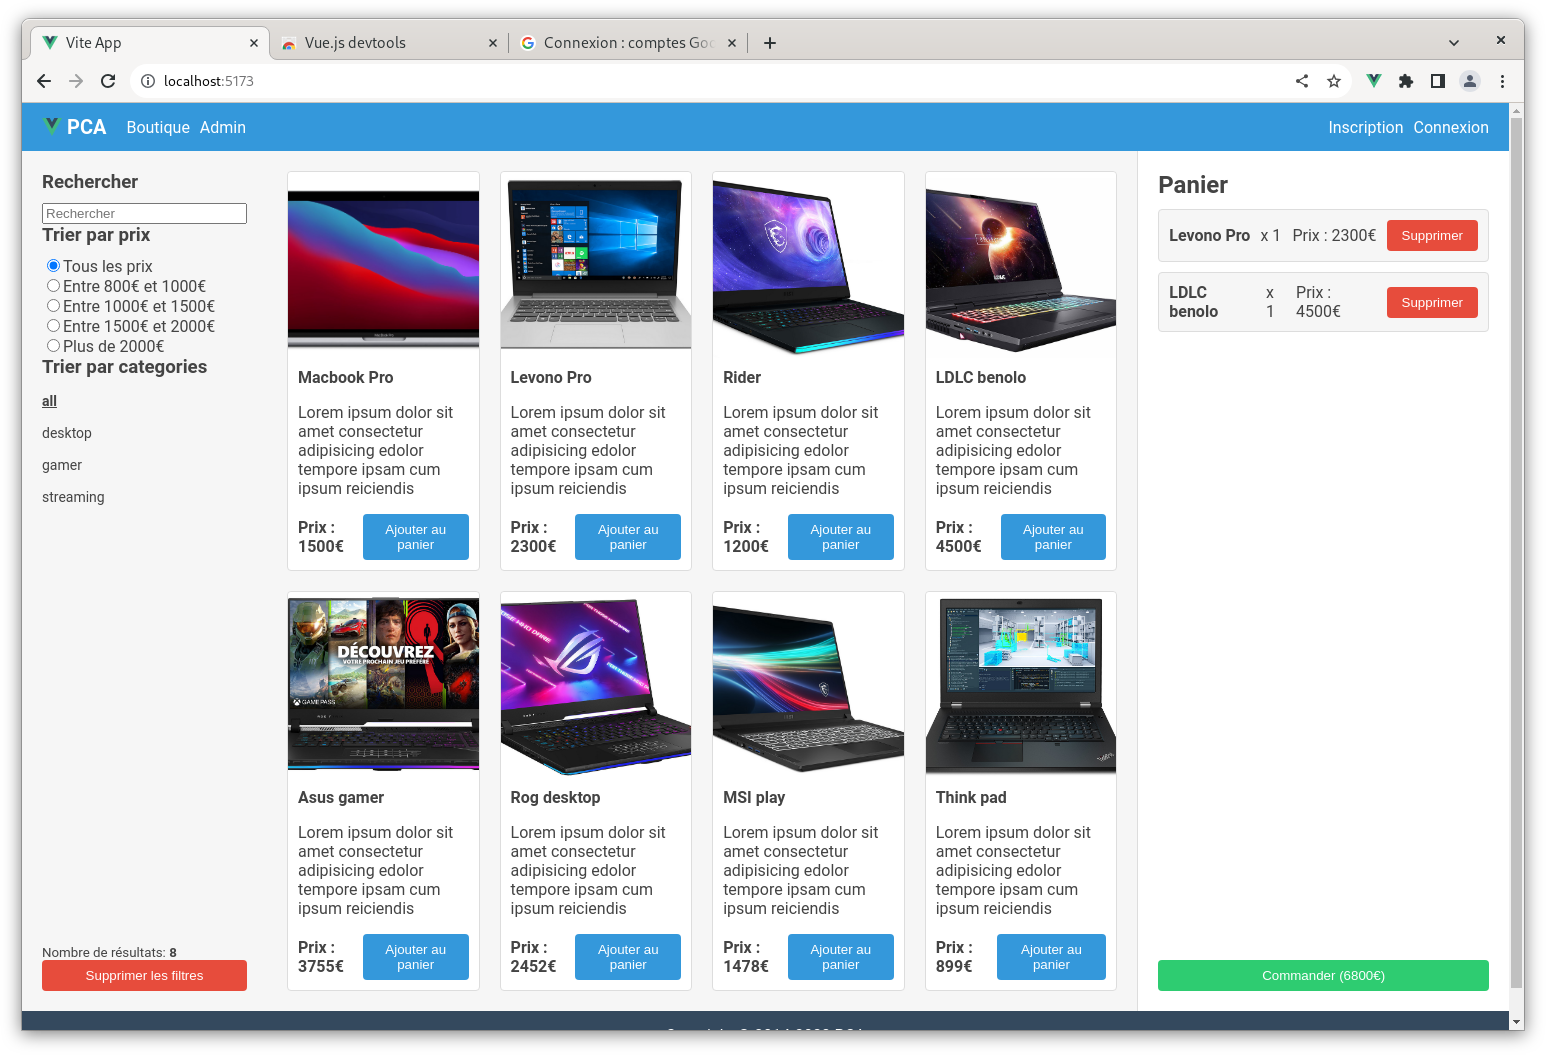
\includegraphics[width=15cm]{images/image28.png}
\end{center}
